%% ---------------------------------------------------------------------
\section{Hardware description and system architecture}
\label{sec:arch}

\subsection{Overview}

The system is split across two computers joined by an IEEE~802.11 link
(\cref{fig:system}). The \emph{airborne segment} contains the flight controller, which
keeps sole authority over attitude stabilisation and motor mixing, and a Raspberry Pi
companion computer that only moves data. It reads the autopilot over MAVLink, the
LiDAR over a USB--serial bridge and the camera over USB Video Class (UVC), and
forwards velocity commands back to the autopilot. The \emph{ground segment} is a
laptop with an NVIDIA GPU running ROS~2 Humble. It performs state reconstruction,
mapping, planning, perception, visualisation and health monitoring.

This division follows from three engineering constraints. (i) The inner control loop
must not depend on the radio link: if Wi-Fi fails the autopilot continues to stabilise
and its own failsafes apply. (ii) The perception workload, roughly \SI{30}{\milli\second}
per frame on a laptop GPU (\cref{sec:val-seg}), is far beyond a Raspberry Pi CPU at
useful frame rates. (iii) During development every intermediate signal should be
observable in RViz and PlotJuggler without loading the vehicle.

\begin{figure}[t]
\centering
\begin{tikzpicture}[x=1cm, y=1cm]
  % ---------------- airborne segment
  \node[ext, minimum width=20mm] (rc)  at (0.2, 1.0) {RC receiver\\(pilot)};
  \node[ext, minimum width=20mm] (esc) at (0.2,-1.0) {ESCs\\+ motors};
  \node[hw, minimum width=33mm] (imu)  at (3.7, 1.35) {IMU, baro, compass (FMU)};
  \node[hw, minimum width=36mm] (fc)   at (3.7, 0.0) {Flight controller\\Pixhawk 6C, ArduPilot EKF3};
  \node[hw, minimum width=33mm] (flow) at (3.7,-1.35) {Optical flow + rangefinder};
  \node[hw, minimum width=28mm, minimum height=24mm] (pi) at (8.4, 0.0)
       {\textbf{Raspberry Pi}\\companion\\[2pt]\scriptsize\code{start_streams.py}};
  \node[hw, minimum width=26mm] (lidar) at (12.2, 0.75) {YDLIDAR G2\\2D LiDAR};
  \node[hw, minimum width=26mm] (cam)   at (12.2,-0.75) {USB camera\\UVC, MJPEG};
  \draw[arr] (imu) -- (fc);
  \draw[arr] (flow) -- (fc);
  \draw[arr] (rc) -- (fc.west |- rc);
  \draw[arr] (fc.west |- esc) -- (esc);
  \draw[darr] (fc) -- node[lbl,above]{USB} node[lbl,below,yshift=-1pt]{MAVLink} (pi);
  \draw[arr] (lidar) -- node[lbl,above]{USB} (pi.east |- lidar);
  \draw[arr] (cam) -- node[lbl,below]{USB} (pi.east |- cam);
  \begin{scope}[on background layer]
    \node[grp, fit=(rc)(esc)(imu)(flow)(pi)(lidar)(cam)] (air) {};
  \end{scope}
  \node[font=\footnotesize\bfseries, anchor=south west] at (air.north west) {Airborne segment};

  % ---------------- radio link
  \node[draw=blk1!70!black, fill=blk1!6, minimum width=15.0cm, minimum height=5mm,
        font=\footnotesize\itshape] (wifi) at (6.45,-3.0) {Wi-Fi 802.11 link (direct, e.g.\ laptop 5\,GHz hotspot)};
  \draw[darr] (pi.south) -- (pi.south |- wifi.north);

  % ---------------- ground segment
  \def\ry{-4.55}
  \node[sw, font=\scriptsize, minimum width=30mm] (cb) at (0.75,\ry)  {\code{mavlink_cmd_bridge}};
  \node[sw, font=\scriptsize, minimum width=30mm] (lr) at (4.55,\ry)  {\code{lidar_udp_receiver}};
  \node[sw, font=\scriptsize, minimum width=30mm] (br) at (8.35,\ry)  {\code{mavlink_to_ros2_bridge}};
  \node[sw, font=\scriptsize, minimum width=30mm] (cr) at (12.15,\ry) {\code{camera_tcp_receiver}};
  \draw[arr, blk2!90!black] (cb.north) -- node[lbl,right]{UDP 14553} (cb.north |- wifi.south);
  \draw[arr, blk1] (lr.north |- wifi.south) -- node[lbl,right]{UDP 14552} (lr.north);
  \draw[arr, blk1] (br.north |- wifi.south) -- node[lbl,right]{UDP 14551} (br.north);
  \draw[arr, blk1] (cr.north |- wifi.south) -- node[lbl,right]{TCP 5000} (cr.north);

  \node[sw, minimum width=40mm, minimum height=11mm] (nav) at (6.45,-6.35)
       {\textbf{Nav2}: rolling costmaps,\\NavFn planner, DWB controller};
  \node[sw, minimum width=28mm, minimum height=11mm] (seg) at (12.15,-6.35)
       {YOLOv8 + SAM~2.1\\(GPU)};
  \draw[arr] (lr.south) -- node[lbl,left]{\topic{/scan}} (lr.south |- nav.north);
  \draw[arr] (br.south) -- node[lbl,right]{\topic{/odom}, TF} (br.south |- nav.north);
  \draw[arr] (cr) -- node[lbl,right]{\topic{/camera/image_raw}} (seg);
  \draw[arr, blk2!90!black] (nav.west) -| node[lbl,pos=0.3,below]{\topic{/cmd_vel}} (cb.south);
  \node[sw, minimum width=150mm, fill=softgray, draw=black!40] (mon) at (6.45,-7.75)
       {\code{metrics_monitor} (\topic{/metrics/*}, \topic{/diagnostics}) \quad
        \code{scan_to_3d} (\topic{/map_3d}) \quad RViz};
  \begin{scope}[on background layer]
    \node[grp, fit=(cb)(lr)(br)(cr)(nav)(seg)(mon)] (gnd) {};
  \end{scope}
  \node[font=\footnotesize\bfseries, anchor=north west] at (gnd.south west)
       {Ground segment: laptop, Ubuntu 22.04, ROS~2 Humble};
\end{tikzpicture}
\caption{System architecture of the implemented prototype. Blue: hardware; green:
ground software nodes; orange: actuators and pilot input. Blue links carry sensor data
down, the orange link carries velocity commands up. The autopilot retains the inner
attitude loop and failsafes, so loss of the Wi-Fi link never removes stabilisation.}
\label{fig:system}
\end{figure}

\subsection{Airborne hardware}

\Cref{fig:hwphoto} shows the assembled prototype with each component labelled.

\begin{figure}[t]
\centering
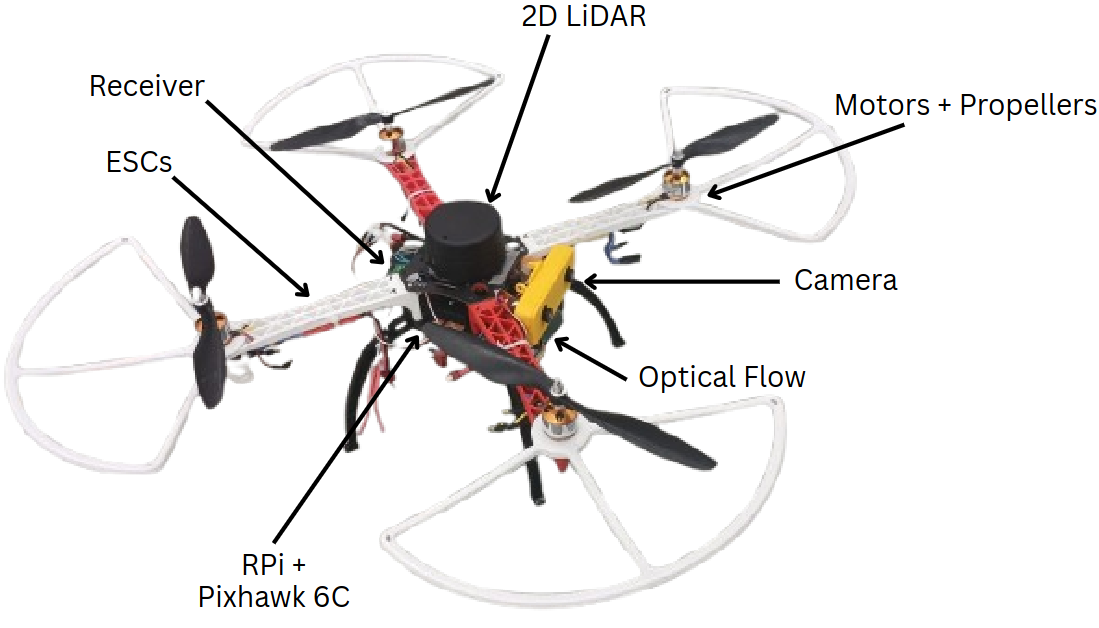
\includegraphics[width=0.9\textwidth]{hardware_pic.png}
\caption{The assembled prototype quadcopter. A 2D LiDAR sits on top of the frame. The
camera and the downward optical-flow sensor are on the front arm. The Raspberry Pi
companion computer and the Pixhawk~6C flight controller are in the centre stack, with
the RC receiver and the ESCs on the frame. Propeller guards are fitted for indoor and
near-obstacle flights.}
\label{fig:hwphoto}
\end{figure}

\paragraph{Flight controller} A Holybro Pixhawk~6C running ArduPilot (ArduCopter)
provides attitude estimation and control, the EKF3 navigation
filter, the motor mixer, RC input and failsafes. It is connected to the companion by
USB. A UART on \code{/dev/serial0} is also supported, provided the baud rate matches
\code{SERIALx_BAUD}. Persistent device naming is provided by udev rules that map the
USB vendor/product identifiers of common Pixhawk, Holybro, CubePilot and STM32 FMU
boards to \code{/dev/pixhawk} (\code{raspberry_pi/99-pixhawk.rules}). The software also
supports PX4 for discovery and mode handling, but the deployed command path targets
ArduPilot \code{GUIDED} mode.

\paragraph{Downward optical flow and rangefinder} We use an MTF-01 flow/range
module connected to the autopilot.
Its data reach the companion as MAVLink \code{OPTICAL_FLOW} and \code{DISTANCE_SENSOR}
messages. The companion software converts the flow to metric body velocity
(\cref{eq:flow-ap}) and uses the range as the preferred height source.

\paragraph{2D LiDAR} A YDLIDAR G2 triangulation LiDAR connected through its USB--serial
adapter at 115\,200 baud. The Pi parses the native packet protocol directly (sync
\code{0xAA55}, start/end angles, three-byte samples), bins returns into 360 one-degree
cells, and accepts ranges in \SIrange{0.12}{16}{\metre}. The FTDI low-latency flag is
set so the adapter does not batch bytes for up to \SI{16}{\milli\second}. We measured the sensor
turning at 6.4 revolutions per second. The transform used for the
mount is $\,^{b}\mathbf{T}_{l}=(0,0,\SI{-0.15}{\metre})$ with zero rotation. This is an estimate and should
be measured on each airframe (\cref{sec:build-calib}).

\paragraph{Camera} A USB~2.0 UVC camera (Arkmicro \code{18ec:3399} on the prototype;
Logitech, ELP and OpenMV identifiers are also mapped to \code{/dev/camera}) is forced
into MJPEG at 640$\times$480. Uncompressed YUYV at that size saturates USB~2.0 and
lowers the frame rate. The forward-looking mount is modelled as
$\,^{b}\mathbf{T}_{c}=(\SI{0.10}{\metre},0,\SI{0.05}{\metre})$, again an estimate.

\paragraph{Companion computer} A Raspberry Pi~5 (4\,GB) running Linux and plain Python~3. Its only
dependencies are \code{pymavlink}, \code{pyserial}, OpenCV and NumPy. ROS is not
required on the vehicle. Setup installs udev rules, serial-group access,
\code{chrony} and \code{iw}, and grants passwordless use of exactly the
\code{iw ... power_save off} and \code{chronyc} commands the supervisor needs.

\paragraph{Pilot link} The RC receiver connects directly to the autopilot, so the pilot
can always override autonomy by switching out of \code{GUIDED}. The
receiver is a RadioMaster RP1 V2 on ExpressLRS.

\paragraph{Airframe, propulsion and power} The vehicle is built on a standard F450
quadrotor kit (\SI{450}{\milli\metre} diagonal, glass-fibre plates, polyamide arms) with
propeller guards (\cref{fig:hwphoto}). Each arm carries a A2212
\SI{1000}{KV} brushless motor driven by a \SI{30}{\ampere} SimonK ESC and a
10$\times$4.5\,in (1045) propeller. A 3S \SI{2200}{\milli\ampere\hour} LiPo powers
the vehicle through the autopilot power module. The bench log in \cref{sec:val-bench}
was recorded with no flight battery connected (reported voltage \SI{0.19}{\volt}).

\subsection{Electrical interconnection}

\Cref{fig:wiring} gives the interconnection schematic at connector level. On the
airborne side all companion connections are USB, which removes the need for level
shifting or custom wiring between the Pi and its peripherals and makes the set-up
reproducible with stock cables. The 3S pack feeds the ESCs and, through the
power module, the autopilot; the Pi takes a separate \SI{5}{\volt} regulator.

\begin{figure}[t]
\centering
\begin{tikzpicture}[x=1cm, y=1cm, font=\footnotesize,
    box/.style={draw, thick, align=center, rounded corners=1pt},
    pwr/.style={very thick, red!70!black},
    usb/.style={thick, blk1!80!black},
    sig/.style={thick}]
  \node[box, fill=blk2!8, minimum width=18mm, minimum height=36mm] (bat) at (0,-0.2) {3S LiPo\\2200\,mAh};
  \node[box, fill=softgray, minimum width=22mm, minimum height=10mm] (pm)  at (3.4, 1.2) {Power module\\(V/I sense)};
  \node[box, fill=softgray, minimum width=22mm, minimum height=10mm] (bec) at (3.4,-1.6) {5\,V regulator\\($\ge$\SI{3}{\ampere})};
  \node[box, fill=blk2!8, minimum width=22mm, minimum height=9mm]  (esc) at (3.4, 3.4) {4$\times$ 30\,A ESC\\+ A2212 motors};
  \node[box, fill=blk1!8, minimum width=36mm, minimum height=24mm] (fmu) at (8.0, 1.6)
       {\textbf{Pixhawk 6C}\\[2pt]POWER, USB\\RC IN, MAIN OUT 1--4\\I\textsuperscript{2}C / UART};
  \node[box, fill=blk1!8, minimum width=36mm, minimum height=18mm] (pi) at (8.0,-2.0)
       {\textbf{Raspberry Pi}\\[2pt]5\,V input\\USB-A ports, Wi-Fi};
  \node[box, fill=softgray, minimum width=24mm] (rx)    at (13.0, 2.4) {RC receiver};
  \node[box, fill=softgray, minimum width=24mm] (flow)  at (13.0, 0.9) {Flow / range\\module};
  \node[box, fill=softgray, minimum width=24mm] (lidar) at (13.0,-1.4) {YDLIDAR G2\\(USB adapter)};
  \node[box, fill=softgray, minimum width=24mm] (cam)   at (13.0,-2.7) {USB camera};

  \draw[pwr] (bat.east |- pm) -- node[above,font=\scriptsize]{V\textsubscript{bat}} (pm.west);
  \draw[pwr] (bat.east |- bec) -- node[above,font=\scriptsize]{V\textsubscript{bat}} (bec.west);
  \draw[pwr] (pm.north) -- node[right,font=\scriptsize]{V\textsubscript{bat}} (esc.south);
  \draw[pwr, thick] (pm.east) -- node[above,font=\scriptsize]{5\,V + sense} (fmu.west |- pm.east);
  \draw[pwr, thick] (bec.east) -- node[above,font=\scriptsize]{5\,V} (pi.west |- bec.east);
  \draw[sig] (fmu.north) |- node[pos=0.75,above,font=\scriptsize]{PWM / DShot} (esc.east);
  \draw[sig] (rx.west) -- node[above,font=\scriptsize]{RC} (fmu.east |- rx.west);
  \draw[sig] (flow.west) -- node[below,font=\scriptsize]{I\textsuperscript{2}C/UART} (fmu.east |- flow.west);
  \draw[usb] (fmu.south) -- node[right,font=\scriptsize,align=left]{USB (MAVLink)} (pi.north);
  \draw[usb] (lidar.west) -- node[above,font=\scriptsize]{USB} (pi.east |- lidar.west);
  \draw[usb] (cam.west) -- node[above,font=\scriptsize]{USB} (pi.east |- cam.west);

  \node[anchor=west, font=\scriptsize] at (-0.9,-3.6)
    {\textcolor{red!70!black}{\rule[0.5ex]{6mm}{1.4pt}}~power\qquad
     \textcolor{blk1!80!black}{\rule[0.5ex]{6mm}{1pt}}~USB data\qquad
     \rule[0.5ex]{6mm}{0.8pt}~signal};
\end{tikzpicture}
\caption{Connector-level interconnection schematic of the prototype. A Raspberry Pi with USB
peripherals should be supplied from a regulator rated at least \SI{3}{\ampere}, not
from the autopilot's servo rail.}
\label{fig:wiring}
\end{figure}

\subsection{Network interface}

Each data stream uses its own transport and port (\cref{tab:ports}). Only one process
may bind a given laptop port, so the stand-alone (ROS-free) laptop tools are used
\emph{instead of}, not alongside, the ROS stack.

\begin{table}[H]
\centering\small
\caption{Pi--laptop interface (from \code{docs/REFERENCE.md} and the source).}
\label{tab:ports}
\begin{tabularx}{\textwidth}{l l l >{\raggedright\arraybackslash}p{3.3cm} L}
\toprule
\textbf{Stream} & \textbf{Dir.} & \textbf{Transport} & \textbf{Encoding / QoS} & \textbf{Endpoints $\rightarrow$ ROS topic} \\
\midrule
Telemetry & Pi$\rightarrow$L & UDP 14551 & JSON $\le$\SI{1400}{B}, DSCP CS6 & \code{telemetry_streamer.py} $\rightarrow$ \code{mavlink_to_ros2_bridge} $\rightarrow$ \topic{/odom}, TF \\
Raw MAVLink & Pi$\rightarrow$L & UDP 14550 & MAVLink v2 & monitoring only (e.g.\ QGroundControl) \\
LiDAR & Pi$\rightarrow$L & UDP 14552 & binary \SI{1094}{B}, DSCP CS6 & \code{lidar_udp_streamer.py} $\rightarrow$ \code{lidar_udp_receiver} $\rightarrow$ \topic{/scan} \\
Camera & Pi$\rightarrow$L & TCP 5000 & JPEG + JSON header, DSCP AF41 & \code{camera_streamer.py} $\rightarrow$ \code{camera_tcp_receiver} $\rightarrow$ \topic{/camera/image_raw} \\
Velocity & L$\rightarrow$Pi & UDP 14553 & JSON, DSCP CS6 & \code{mavlink_cmd_bridge} $\rightarrow$ \code{mavlink_cmd_listener.py} \\
Mode/arm & L$\rightarrow$Pi & UDP 14552 & JSON & \code{mavlink_cmd_bridge} $\rightarrow$ \code{telemetry_streamer.py} \\
\bottomrule
\end{tabularx}
\end{table}

\subsection{Software architecture}

\paragraph{Airborne processes} \code{start_streams.py} is the single entry point on
the Pi. It launches and supervises three child processes (telemetry, LiDAR, camera),
restarts any that exit with back-off, and optionally (\code{--nav-cmds}) runs the
velocity listener \emph{inside} the telemetry process so that it shares that process's
MAVLink connection; only one process can own the autopilot's serial port. On start it also disables Wi-Fi power saving on the interface that routes
to the laptop (re-checked every \SI{30}{\second}) and adds the laptop as the preferred
\code{chrony} time source. Both changes are reverted on exit.

\paragraph{Ground ROS~2 packages} \Cref{tab:packages} lists the workspace packages. A
single launch file, \code{navigation_real.launch.py}, starts the bridge nodes, static
transforms, Nav2, perception, the 3D mapper, the metrics monitor and RViz.

\begin{table}[H]
\centering\small
\caption{ROS~2 workspace packages.}
\label{tab:packages}
\begin{tabularx}{\textwidth}{l L}
\toprule
\textbf{Package} & \textbf{Role} \\
\midrule
\code{gps_denied_bridge} & Pi$\leftrightarrow$ROS bridge: telemetry$\rightarrow$\topic{/odom}+TF, LiDAR$\rightarrow$\topic{/scan}, camera, \topic{/cmd_vel}$\rightarrow$Pi, health metrics, 3D voxel mapping \\
\code{x500_navigation} & Nav2 parameter sets (real, office, Baylands), SLAM configs, launch files, RViz layouts, drone behaviour tree, office world generator \\
\code{quadcopter_perception} & Hybrid YOLO + SAM segmentation node and ROS-independent core, unit tests \\
\code{x500_px4_bridge} & Simulation: Nav2 $\rightarrow$ PX4 OFFBOARD bridge with LiDAR safety filter; Gazebo Harmonic transport bridge; TF broadcaster \\
\code{quadcopter_bringup} & Simulation bring-up and keyboard/GUI teleoperation \\
\code{quadcopter_localization}, \code{quadcopter_mapping} & Early work (VO$\rightarrow$PX4 parameters, frame utilities; mapping stub) \\
\code{m-explore-ros2}, \code{px4_msgs} & Third-party: frontier exploration \cite{hoerner2016mapmerge}, PX4 message definitions \\
\bottomrule
\end{tabularx}
\end{table}

\subsection{Coordinate frames}
\label{sec:frames}

ROS uses an East--North--Up (ENU) world frame and a Forward--Left--Up (FLU) body
frame \cite{rep103,rep105}. ArduPilot and PX4 use North--East--Down (NED) and
Forward--Right--Down (FRD). All conversions take place at the bridge boundary, so the
rest of the stack sees a single convention (\cref{fig:tf}).

\begin{figure}[H]
\centering
\begin{tikzpicture}[node distance=4mm and 9mm, font=\footnotesize]
  \node[blk, fill=softgray] (map) {\code{map}};
  \node[blk, fill=softgray, right=13mm of map] (odom) {\code{odom}};
  \node[blk, fill=blk1!10, right=of odom] (base) {\code{base_link}};
  \node[blk, fill=blk3!10, above right=1mm and 9mm of base] (laser) {\code{laser_frame}};
  \node[blk, fill=blk3!10, below right=1mm and 9mm of base] (cam) {\code{camera_frame}};
  \draw[arr, dashed] (map) -- node[lbl,above]{SLAM} (odom);
  \draw[arr] (odom) -- node[lbl,above]{bridge} (base);
  \draw[arr] (base) -- node[lbl,above,sloped]{static} (laser);
  \draw[arr] (base) -- node[lbl,below,sloped]{static} (cam);
\end{tikzpicture}
\caption{Transform tree on the real vehicle. \code{odom}$\rightarrow$\code{base_link}
is broadcast by \code{mavlink_to_ros2_bridge}. Sensor mounts are static transforms.
In the real configuration Nav2 operates in \code{odom} (rolling costmaps, no global map).
The simulation adds \code{map}$\rightarrow$\code{odom} from SLAM~Toolbox and a
\code{base_footprint} frame for 2D planning.}
\label{fig:tf}
\end{figure}
